\chapter{Řešená úloha}\label{problem}

Řešená úloha je problémem binární klasifikace, tedy problém, kdy je cílem zařadit objekty do jedné ze dvou tříd, jež nazýváme pozitivní a negativní. Tedy cílem je navrhnout vhodnou klasifikační funkci, který pro daný vstupní objekt určí příslušnou třídu. Vstupními objekty jsou v tomto případě adresy URL (srov. \cite{berners-lee_uniform_1994}). Příklad takovéto adresy je na obrázku \ref{url}. \BPname{Negativní třídou} se rozumí veškerý síťový provoz, který je součástí běžného provozu uživatele-klienta a jím spuštěných programů. \BPname{Pozitivní třídou} se rozumí síťový provoz který pochází z aktivit malware a nežádoucího software.

\begin{figure}[h]
	\caption{Adresa URL}\label{url}
	\centering
	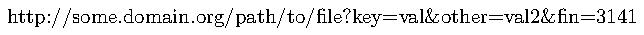
\includegraphics{images/url/url.pdf}
\end{figure}

Adresa URL se skládá z několika částí, mezi běžné patří \BPname{protokol} (\BPenname{protocol}), \BPname{doména} (\BPenname{domain} nebo \BPenname{host}), \BPname{port}, \BPname{cesta} (\BPenname{path}), \BPname{dotaz} (\BPenname{query} nebo \BPenname{searchpart}). Vzhledem k tomu, že protokolů je relativně málo a port se ve většině případů neudává, lze tyto dvě části pominout a zabývat se pouze doménou, cestou a dotazem.

\section{Struktura adresy URL}\label{URL_structure}

\cite{berners-lee_uniform_1994} definuje abecedu (dále označovanou \( \Sigma \)) všech možných znaků v adrese URL jako malá a velká písmena anglické abecedy, čísla a znaky \$ - \_ . + ! * ' ( ) , \% ; / ? : @ \& =. Každá adresa URL je pak slovem abecedy \( \Sigma \) (ne však naopak). Vybrané tři části adresy URL jsou definovány následovně.
\begin{define}
	\BPname{Doména} je podslovem adresy URL konstruovaným následovně: Pokud adresa URL obsahuje podslovo "://", doména začíná za tímto podslovem. V opačném případě doména začíná na záčátku adresy URL. Doména končí před prvním výskytem znaku "/" po začátku domény, případně na konci adresy URL, pokud tato už žádný znak "/" neobsahuje.
\end{define}
\begin{define}
	Pokud je doména sufixem adresy URL, je \BPname{cesta} definována jako prázdné slovo. V opačném případě je cesta definována jako podslovo adresy URL, začínající za znakem "/" ukončujícím doménu. Cesta končí před prvním výskytem znaku "?" po začátku cesty, případně na konci adresy URL, pokud tato už žádný znak "?" neobsahuje.
\end{define}
\begin{define}
	Pokud je doména nebo cesta sufixem adresy URL, je \BPname{dotaz} definován jako prázdné slovo. V opačném případě je dotaz definován jako sufix adresy URL, začínající za za znakem "?" ukončujícím cestu.
\end{define}

\begin{figure}[h]
	\caption{Části adresy URL}\label{url_parts}
	\centering
	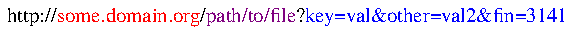
\includegraphics{images/url_parts/url_parts.pdf}
\end{figure}

Na obrázku \ref{url_parts} je příklad dělení adresy URL. Doména ja zvýrazněná červenou barvou, cesta fialovou a dotaz modrou.

Každá z těchto tří částí adresy URL se sama skládá z několika podčástí. Doména se skládá z několika úrovní, lišících se obecností. Tyto části jsou odděleny znakem ".". Cesta se skládá z názvů složek a souborů, které jsou dotazovány. Tyto části jsou odděleny znakem "/". Dotaz je tvořen dvojicemi klíč--hodnota, oddělenými znakem "\&". Na obrázku \ref{url_subparts} je příklad těchto podčástí, v barvách korespondujících s obrázkem \ref{url_parts}, v různých odstínech pro různé podčásti.

\begin{figure}[h]
	\caption{Podčásti adresy URL}\label{url_subparts}
	\centering
	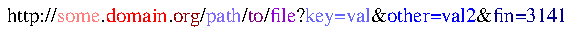
\includegraphics{images/url_subparts/url_subparts.pdf}
\end{figure}

Je zřejmé, že na pořadí podčástí domény záleží, definují "cestu" k cílovému serveru a jsou řazeny od nejkonkrétnější k nejobecnější (srov. \cite{mockapetris_domain_1987}).	Stejně tak u cesty závisí na pořádí, které definuje adresářové umístění požadovaného souboru na serveru.

\section{Proč MIL?}

Pro modelování klasifikační funkce byl využit přístup pomocí tzv. \BPname{Multi-instančního učení} (MIL)\footnote{resp. jeho speciální varianta, blíže popsaná v kapitole \ref{model}}, poprvé popsaného v \cite{dietterich_solving_1997}. Tento přítup, podrobněji popsaný v kapitole \ref{MIL}, vychází z předpokladu, že vstupem klasifikační funkce není jedna instance, ale sada (neznámého počtu) instancí, které všechny dohromady tvoří jeden vzorek, zvaný \BPname{taška}. Dále je pak předpokládáno, že každou tašku je možno zařadit do nějaké třídy, přestože ne všechny instance odpovídají této třídě. Adresu URL lze považovat za takovouto tašku za využití jejího hierarchického modelu, nastíněného v sekci \ref{URL_structure}. Proto lze přístup pomocí Multi-instančního učení aplikovat na tento problém.

Přístup pomocí Multi-instančního učení produkuje topologicky složitější modely než je srovnatelný klasický model. Výměnou za tuto nevýhodu v podobě zvětšené složitosti implementační je zmenšená složitost implementační. Multi-instanční model totiž modeluje každou instanci nejprve zvlášť a teprve poté následuje model pro celý vzorek. To v případě použití neuronové sítě znamená výrazně méné propojení než u srovnatelné klasické síťě se stejnými počty neuronů ve stejných vrstvách. Důležitým rozdílem též je, že narozdíl od klasického modelu je Multi-instanční model rozdělen do dvou částí (model pro instance a model pro tašky), přičemž ten samý instanční model je použit několikrát v rámci jedné tašky.

Multi-instanční přístup nám tedy dovoluje vytvořit model, jehož topologie odpovídá hierarchické struktuře adresy URL, je výpočetně méně náročný než srovnatelný klasický model a umožňuje znovupoužití některých částí. To jsou důvody, proč byl tento přístup zvolen.

\section{Trénovací a testovací data}

\todo{Napsat}
